% ---------------------------------------------------------------------
% Basic configuration of Beamera and Jagiellonian
% ---------------------------------------------------------------------
\RequirePackage[l2tabu, orthodox]{nag}



\ifx\PresentationStyle\notset
\def\PresentationStyle{dark}
\fi



\documentclass[10pt,t]{beamer}
\mode<presentation>
\usetheme[style=\PresentationStyle,logoLang=Latin,logoColor=monochromaticJUwhite,JUlogotitle=yes]{jagiellonian}



% ---------------------------------------
% Configuration files of Jagiellonian loceted in catalog preambule
% ---------------------------------------
\input{./preambule/LanguageSettings/JagiellonianPolishLanguageSettings.tex}
\input{./preambule/TextposConfiguration/TextposConfiguration.tex}

\input{./preambule/JagiellonianCustomizationGeneral.tex}
\input{./preambule/JagiellonianCustomizationCommands.tex}










% ---------------------------------------
% Packages, libraries and their configuration
% ---------------------------------------
\usepackage{mathcommands}





% ---------------------------------------
% Configuration for this particular presentation
% ---------------------------------------
\usetikzlibrary{arrows.meta}

\tikzstyle{axis arrow} = [-{Straight Barb[scale=1.2]},thick]


% % Autor: Kamil Ziemian

% % ---------------------------------------------------------------------
% % Podstawowe ustawienia Beamera i używane pakiety
% % ---------------------------------------------------------------------
% \RequirePackage[l2tabu, orthodox]{nag}  % Wykrywa przestarzałe i niewłaściwe
% % sposoby używania LaTeXa. Więcej jest w l2tabu English version.

% \documentclass[10pt,t]{beamer}  % Klasa dokumentu
% \mode<presentation>  % Rodzaj tworzonych slajdów Beamera
% \usetheme[style=dark]{jagiellonian}  % Temat graficzny



% % General configuration of jagiellonian
% \input{./preambule/JagiellonianConfiguration/JagiellonianCoreConfiguration.tex}
% \input{./preambule/JagiellonianCustomization.tex}


% \usepackage{tikz}


% \usepackage{csquotes}


% % ------------------------------
% % Pakiet "hyperref" Polecano by umieszczać go na końcu preambuły.
% % ------------------------------
% \usepackage{hyperref}  % Pozwala tworzyć hiperlinki i zamienia odwołania
% % do bibliografii na hiperlinki.



% % ------------------------------
% % Pakiety napisane przez użytkownika.
% % Mają być w tym samym katalogu to ten plik .tex
% % ------------------------------
% \usepackage{latexshortcuts}
% \usepackage{mathshortcuts}



% % ------------------------------
% % Pakiet "hyperref"
% % Polecano by umieszczać go na końcu preambuły.
% % ------------------------------
% \usepackage{hyperref}  % Pozwala tworzyć hiperlinki i zamienia odwołania
% % do bibliografii na hiperlinki.









% ---------------------------------------------------------------------
% Tytuł, autor, data
\title{Promieniowanie Hawkinga czarnej dziury powstałej w~wyniku sferycznie
  symetrycznego kolapsu}
\subtitle{Seminarium Astrofizyczne}

\author{Kamil Ziemian \\
  \texttt{kziemianfvt@gmail.com}}


\institute{Zakład Teorii Pola, \\
  Uniwersytet Jagielloński w~Krakowie}

\date[19 maja 2021~r.]{19 maja 2021~r.}
% ---------------------------------------------------------------------










% ####################################################################
\begin{document}
% ####################################################################





% Wyrównanie do lewej z łamaniem wyrazów

\RaggedRight





% ######################################
\maketitle % Tytuł całego tekstu
% ######################################





% ##################
\begin{frame}
  \frametitle{Plan wystąpienia}


  \tableofcontents

\end{frame}
% ##################





% ######################################
\section{Wprowadzenie i zarys historyczny}
% ######################################



% ##################
\begin{frame}
  \frametitle{Uwagi ogólne}


  \begin{itemize}

  \item W~większości wzorów przyjąłem, że wszystkie stałe fizyczne są
    równe $1$. $c = 1$, $\hbar = 1$, $G = 1$.

  \item Pozwoliłem sobie przetłumaczyć część przytaczanych wyników na
    bardziej standardowy formalizm, który, mam nadzieję, jest bardziej
    przystępny.

  \item Czy mam przypomnieć, co to jest grawitacja powierzchniowa?

  \item Pierwsza część wystąpienia idzie w porządku historycznym.

  \item Dla wygody wszystkie pola są bezmasowe: $m = 0$.

  \item Zdaję sobie sprawę, że seminarium ma wiele niedociągnięć,
    dlatego proszę przerywać i~zadawać pytania.

  \item Mam przygotowanych kilka slajdów dodatkowych, zawierających
    informacje, które musiałem usunąć z~głównej części.

  \item Na górze slajdu jest pasek pokazujący, w której części
    seminarium jesteśmy.

  \item Mogę przesłać \textsc{pdf} seminarium każdemu kto o to
    poprosi.

  \end{itemize}

\end{frame}
% ##################





% ##########
\begin{frame}
  \frametitle{Grawitacja powierzchniowa (ang. \textit{surface gravity})}


  Rozważmy statyczną, osiowo symetryczną, asymptotycznie płaską
  czasoprzestrzeń z~obecną w niej czarną dziurą. W takiej
  czasoprzestrzeni istnieją dwa pola~Killinga:
  $K^{ \mu }$~odpowiedzialne za~przesunięcie w~czasie
  i~$\widetilde{ K }^{ \mu }$ odpowiedzialne za~obroty przestrzenne.
  Istnienie przestrzennopodobnego pola Killinga $\tilde{ K }^{ \mu }$
  pozwala nam wybrać asymptotycznie płaską hiperpowierzchnię $B$,
  do~której jest ono styczne i~która przecina horyzont zdarzeń czarnej
  dziury na~dwie części.

  Rozważmy parametr $t$ krzywych całkowych pola $K^{ \mu }$ i~wektor
  świetlny obliczony na horyzoncie zdarzeń:
  \begin{equation}
    \label{eq:Promieniowanie-Hawkinga-01}
    l^{ \mu } =  \frac{ d x^{ \mu } }{ d t }.
  \end{equation}

  Wprowadźmy wektor $n^{ \mu }$ styczny do~hiperpowierzchni $B$
  i~znormalizowany do
  \begin{equation}
    \label{eq:Promieniowanie-Hawkinga-02}
    l^{ \mu } n_{ \mu } = -1.
  \end{equation}

\end{frame}
% ##########





% ##################
\begin{frame}
  \frametitle{Grawitacja powierzchniowa (ang. \textit{surface gravity})}


  Grawitacja powierzchniowa w~określonym punkcie jest zdefiniowana
  jako:
  \begin{equation}
    \label{eq:Promieniowanie-Hawkinga-03}
    \kappa = -\big( \nabla_{ \mu } l_{ \nu } \big) n^{ \mu } l^{ \nu }.
  \end{equation}
  Dla czarnej dziury Schwarzschilda jest ona stała na~całych
  horyzoncie zdarzeń.

  Parametr $\kappa$ wyraża w jakim stopniu $t$ odbiega od parametru
  afinicznego.

\end{frame}
% ##################





% ##################
\begin{frame}
  \frametitle{Cztery prawa mechaniki/termodynamiki czarnych dziur}


  W~pracy \textit{The Four Laws of Black Hole Mechanics} ukończonej
  przed końcem stycznia 1973 roku, James M. Bardeen, Brandon Carter
  i~Stephen W.~Hawking przedstawiają drugie, pierwsze, zerowe
  i~trzecie prawo mechaniki czarnych dziur
  \cite{BardeenCarterHawkingFourLawsOfBHMechanics1973}. Proszę się
  mnie nie pytać, czemu w takiej kolejności.

  Zauważają podobieństwo do praw termodynamiki i~analogię między
  entropią a~powierzchnią czarnej dziur $A$ oraz temperaturą
  a~wielkością $\kappa / 8\pi$, gdzie $\kappa$ to grawitacja
  powierzchniowa. Jednak w~tej pracy jest to tylko analogia.

\end{frame}
% ##################





% ##################
\begin{frame}
  \frametitle{Cztery prawa mechaniki/termodynamiki czarnych dziur}


  „Należy zaznaczyć, że $\kappa / 8\pi$ i~$A$ są różne od prawdziwej
  temperatury i~entropii czarnej dziury.”

  „W rzeczywistości efektywna temperatura czarnej dziury równa jest
  zeru absolutnemu. Jeden ze sposobów by to pokazać polega na
  zauważeniu, że czarna dziura nie może być w~równowadze
  termodynamicznej z ciałem doskonale czarnym o niezerowej
  temperaturze, ponieważ czarna dziura nie może emitować żadnego
  promieniowania, podczas gdy jakieś promieniowanie z zewnątrz zawsze
  będzie przekraczać jej horyzont.”

  Strony 8 pracy, 168 w tomie 31 Commun. Math. Phys.
  \cite{BardeenCarterHawkingFourLawsOfBHMechanics1973}


  Fizyczna interpretacja $A$ jako entropii
  i~$T_{ BH } = \kappa / 2\pi$ jako temperatury czarnej dziury została
  przedstawione przez Jacoba Bekensteina w swojej ukończonej przed
  listopadem 1972 roku pracy \textit{Black Holes and Entropy}
  \cite{BekensteinBlackHolesAndEntropy1973}. W~świetle tego Hawking
  będzie próbował rozwiązać w 1975 roku dzięki uwzględnieniu kwantowej
  teorii pola.

\end{frame}
% ##################










% ######################################
\section{Kwantowanie pola poza czasoprzestrzenią Minkowskiego}
% ######################################



% ##################
\begin{frame}
  \frametitle{Kwantowanie pola poza czasoprzestrzenią Minkowskiego}


  Stephen Fulling, w swojej pracy opublikowanej 1973 roku
  \cite{FullingNonuniquenessOfCanocialFieldQuantizationInRiemannian1973},
  chyba pierwszy zwrócił uwagę na problemy z kwantowaniem pola
  skalarnego poza czasoprzestrzenią Minkowskiego.

  Rozpatrywał on teorię pola skalarnego zdefiniowaną przez gęstość
  lagrangianu:
  \begin{equation}
    \label{eq:Promieniowanie-Hawkinga-04}
    \Lcal( x ) =
    \frac{ 1 }{ 2 } \abs{ g( x ) }^{ \frac{ 1 }{ 2 } }
    g^{ \mu \nu }( x ) \partial_{ \mu } \partial_{ \nu } \widehat{ \phi }( x ).
  \end{equation}
  Dla wygody rozpatruję tylko przypadek bezmasowy: $m = 0$. Prowadzi
  on do oczekiwanych równań ruchu:
  \begin{equation}
    \label{eq:Promieniowanie-Hawkinga-05}
    g^{ \mu \nu }( x ) \nabla_{ \mu } \nabla_{ \nu } \widehat{ \phi }( x ) = 0.
  \end{equation}

\end{frame}
% ##################





% ##################
\begin{frame}
  \frametitle{Kwantowanie pola poza czasoprzestrzenią Minkowskiego}


  Pęd kanoniczny pola wynosi:
  \begin{equation}
    \label{eq:Promieniowanie-Hawkinga-06}
    \widehat{\pi}( x ) =
    \frac{ \partial \Lcal( x ) }{ \partial ( \partial_{ 0 } \widehat{ \phi }( x ) ) }
    = \abs{ g }^{ \frac{ 1 }{ 2 } } g^{ \mu 0 } \partial_{ \mu } \widehat{ \phi }( x ).
  \end{equation}

  Pole kwantowe ma spełniać relacje komutacji:
  \begin{subequations}
    \begin{align}
      \label{eq:Promieniowanie-Hawkinga-07-A}
      &[ \widehat{\phi}( t, \underline{x} ), \widehat{\phi}( t, \underline{y} ) ]
        =
        [ \widehat{\pi}( t, \underline{x} ), \widehat{\pi}( t, \underline{y} ) ]
        = 0 \\
      \label{eq:Promieniowanie-Hawkinga-07-B}
      &[ \widehat{\phi}( t, \underline{x} ), \widehat{\pi}( t, \underline{y} ) ]
        = i \delta( \underline{x} - \underline{y} ), \qquad
        t = x^{ 0 }, \quad \underline{x} = ( x^{ 1 }, x^{ 2 }, x^{ 3 } )
    \end{align}
  \end{subequations}

  Powyższe relacje wedle Fullinga są kowariantne, czyli nie zależą od
  sposobu definicji czasu na zakrzywionej czasoprzestrzeni.

  Fulling podał całkiem naturalny schemat kwantyzacji, który następnie
  zastosował do dwuwymiarowej czasoprzestrzeni Rindlera.

\end{frame}
% ##################





% ##################
\begin{frame}
  \frametitle{Dwuwymiarowa czasoprzestrzeń Rindlera}


  % #############
  \begin{figure}[h]

    \centering

    \begin{tikzpicture}
      \path (-5,0) -- (0,0);


      \draw[dashed,thick] (-1.75,1.75) -- (1.75,-1.75);

      \node at (1.85,1.95) {$t = x$};


      \draw[dashed,thick] (-1.75,-1.75) -- (1.75,1.75);

      \node at (1.85,-1.95) {$t = -x$};


      \draw[axis arrow,color=jAxisBlue] (-2.25,0) -- (2.25,0);

      \node at (2,-0.3) {$x$};


      \draw[axis arrow,color=jAxisBlue] (0,-2.25) -- (0,2.25);

      \node at (0.3,2) {$t$};


      \fill[color=gray,opacity=0.5] (0,0) -- (1.65,1.65) -- (1.65,-1.65)
      -- cycle;


      \node[align=left] at (4,0.8)
      {Czasoprzestrzeń \\
        Rindlera};


      \draw[axis arrow] (2.7,0.8) -- (1.3,0.8);

    \end{tikzpicture}

    \caption{Czasoprzestrzeń Rindlera jest częścią czasoprzestrzeni
      Minkowskiego}

  \end{figure}
  % #############




  Wynik procedury kwantyzacji był dość nieoczekiwany.

\end{frame}
% ##################





% ##################
\begin{frame}
  \frametitle{Kwantowanie pola poza czasoprzestrzenią Minkowskiego}


  Niech $a_{ k }$, $a_{ k }^{ \dagger }$ oznaczają operatory kreacji
  i~anihilacji pola $\widehat{\phi}( x )$ skwantowanego w
  czasoprzestrzeni Rindlera, a~$b_{ k }$, $b_{ k }^{ \dagger }$
  operatory pola skwantowanego w czasoprzestrzeni Minkowskiego.
  Zachodzi relacja:
  \begin{equation}
    \label{eq:Promieniowanie-Hawkinga-08}
    a_{ k } =
    \int\limits_{ -\infty }^{ +\infty } du \, U( k, u ) b_{ u }
    + \int\limits_{ -\infty }^{ +\infty } du \, V( k, u ) b_{ u }^{ \dagger }
  \end{equation}
  Jawna postać $U( k, u )$ i $V( k, u )$ jest znana, dla nas ważne
  jest tylko to, że $V( k, u ) \neq 0$. Co więcej, jeśli oznaczymy
  próżnię kwantyzacji w czp. Rindlera $| 0_{ R } \rangle$, a w~czp. Minkowskiego
  $| 0_{ M } \rangle$ to zachodzi:
  \begin{equation}
    \label{eq:Promieniowanie-Hawkinga-09}
    a_{ k } | 0_{ M } \rangle \neq 0.
  \end{equation}

  Mamy więc $| 0_{ R } \rangle \neq | 0_{ M } \rangle$. To jest problem.

\end{frame}
% ##################





% ##################
\begin{frame}
  \frametitle{Problem z przestrzenią Hilberta}


  W mechanice kwantowej wszystkie przestrzenie Hilberta $\Hcal$
  są ośrodkowe, czyli posiadają przeliczalną ortogonalną bazę. Na
  podstawie jednego z podstawowych twierdzeń teorii przestrzeni
  Hilberta wszystkie są unitarnie równoważne. W~kwantowej teorii pola
  mamy nieośrodkowe przestrzenie Hilberta, które w~ogólności są
  unitarnie nierównoważne.

  W większości przypadków z zależności typu:
  \begin{equation}
    \label{eq:Promieniowanie-Hawkinga-10}
    | 0_{ R } \rangle \neq | 0_{ M } \rangle
  \end{equation}
  wynika, że dwa kwantowe pola $\widehat{\phi}_{ R }( x )$ i
  $\widehat{\phi}_{ M }( x )$ działają na dwie nierównoważne
  przestrzenie Hilberta $\mathcal{H}_{ R }$ i~$\Hcal_{ M }$ są
  to więc dwie \textit{fizycznie} różne teorie.

  W~szczególności „cząstki Rindlera”
  $| k_{ R } \rangle = a_{ k }^{ \dagger } | 0_{ R } \rangle$, wedle
  słów Fullinga, to zupełnie inny jakościowo byt niż „normalne”
  cząstki.

\end{frame}
% ##################





% ##################
\begin{frame}
  \frametitle{Źródło problemu: za mało symetrii}


  Niech $\mathcal{P}$ będzie standardową grupą Poincar\'{e}go. Stan
  próżni $| 0_{ M } \rangle$ ma być nieimiennicza względem działania
  $\mathcal{P}$:
  \begin{equation}
    \label{eq:Promieniowanie-Hawkinga-11}
    \widehat{U}( g ) | 0_{ M } \rangle = | 0_{ M } \rangle, \qquad
    \forall g \in \Pcal,
  \end{equation}
  gdzie $\Ucal( g )$ to operator unitarny implementujący
  transformację Poincar\'{e}go $g$. Ten warunek pozwala nam
  jednoznacznie wybrać nasz stan próżni w czp. Minkowskiego.


  Grupa symetrii czp. Rindlera nie jest grupą $\Pcal$ więc
  patrząc się tylko na jej wewnętrzne własności, nie jesteśmy w stanie
  wybrać jako stanu próżni $| 0_{ M } \rangle$. Chyba że mam
  niewiarygodne szczęście, ale na to nie warto liczyć.

  Więcej informacji można znaleźć w pracy Fulling \textit{Nonuniqueness
    of Canonical Field Quantization in Riemannian Space-Time}
  \cite{FullingNonuniquenessOfCanocialFieldQuantizationInRiemannian1973},
  choć użyta w jej notacja nie zawsze jest najlepsza.

\end{frame}
% ##################





% ##################
\begin{frame}
  \frametitle{Problem \textit{nie} jest krzywina!}


  % #############
  \begin{figure}[h]

    \centering

    \begin{tikzpicture}
      \path (-5,0) -- (0,0);



      \draw[dashed,thick] (-1.75,1.75) -- (1.75,-1.75);

      \node at (1.85,1.95) {$t = x$};


      \draw[dashed,thick] (-1.75,-1.75) -- (1.75,1.75);

      \node at (1.85,-1.95) {$t = -x$};


      \draw[axis arrow,color=jAxisBlue] (-2.25,0) -- (2.25,0);

      \node at (2,-0.3) {$x$};


      \draw[axis arrow,color=jAxisBlue] (0,-2.25) -- (0,2.25);

      \node at (0.3,2) {$t$};


      \fill[color=gray,opacity=0.5] (0,0) -- (1.65,1.65) -- (1.65,-1.65)
      -- cycle;


      \node[align=left] at (4,0.8)
      {Czasoprzestrzeń \\
        Rindlera};


      \draw[axis arrow] (2.7,0.8) -- (1.3,0.8);
    \end{tikzpicture}

    \caption{Czasoprzestrzeń Rindlera jest płaska!}

  \end{figure}
  % #############



  Czasoprzestrzeń Rindlera jest płaska, więc problem \textit{nie} wynika
  z~niezerowej krzywizny, tylko z różnych grup symetrii które
  wybierają różne stany próżni.

\end{frame}
% ##################










% ######################################
\section{Oryginalna analiza Hawkinga}
% ######################################



% ##################
\begin{frame}
  \frametitle{Wracamy do czarnych dziur}


  W swojej pracy \textit{Particle Creation by Black Holes} z 1975 roku
  \cite{HawkingParticleCreationByBlackHole1975}, Hawking nie cytuje
  bezpośrednio artykułu Fullinga, jednak jego idea tłumacząca w~jaki
  sposób pole kwantowe może „znaleźć wyjście” z czarnej dziury opiera
  się na tym co Fulling zaobserwował już dla czp. Rindlera. To zaś
  pozwoli wyjaśnić sprzeczność między niezerową temperaturą czarnej
  dziur a niemożliwością emisji przez nią klasycznego promieniowania
  termicznego.

  W teorii grawitacji Einsteina nie możemy liczyć na grupę symetrii
  tak dużą jak grupa Poincar\'{e}go, więc należy podejrzewać, że różne
  obszary czasoprzestrzeni będą miały różne swoje stany próżni, tym
  samym różne znaczenie tego czym jest „cząstka”.

  To co więc na początku było pustą przestrzenią, na końcu może
  zawierać „cząstki” wedle tego co jest nową definicją „bycia
  cząstką”.

\end{frame}
% ##################





% ##################
\begin{frame}
  \frametitle{To nie jest diagram Penrose’a!}

  \vspace{-0.4em}


  % #############
  \begin{figure}[h]

    \centering

    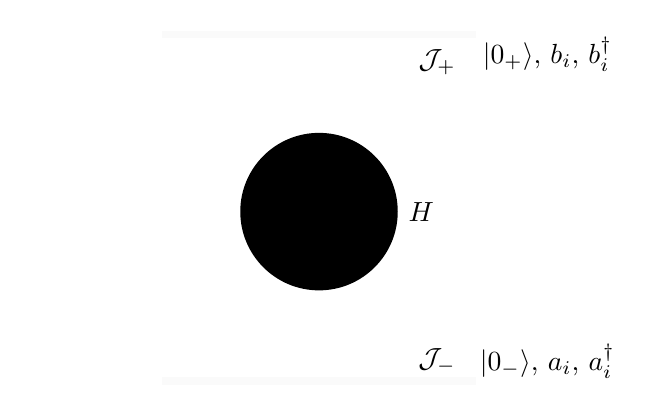
\begin{tikzpicture}
      \path (-3.7,0) -- (0,0);



      \fill[color=white!98!black] (-2,2.2) rectangle +(4,0.1);

      \node at (1.5,1.9) {$\mathcal{J}_{ + }$};

      \node[align=left] at (2.9,2) {$| 0_{ + } \rangle$, $b_{ i }$,
        $b_{ i }^{ \dagger }$};



      \fill[color=black] (0,0) circle [radius=1];

      \node at (1.3,0) {$H$};


      \fill[color=white!98!black] (-2,-2.2) rectangle +(4,0.1);

      \node at (1.5,-1.9) {$\mathcal{J}_{ - }$};

      \node[align=left] at (2.9,-1.9) {$| 0_{ - } \rangle$, $a_{ i }$,
        $a_{ i }^{ \dagger }$};
    \end{tikzpicture}

    \caption{Naiwna ilustracja podejścia Hawkinga}

  \end{figure}
  % #############



  $\Jcal_{ - }$ to nieskończona przeszłość świetlna,
  $\Jcal_{ + }$ to nieskończona przyszłość świetlna, $H$ to
  horyzont czarnej dziury.

\end{frame}
% ##################






% ##################
\begin{frame}
  \frametitle{Promieniowanie czarnej dziury}


  % #############
  \begin{figure}[h]

    \centering

    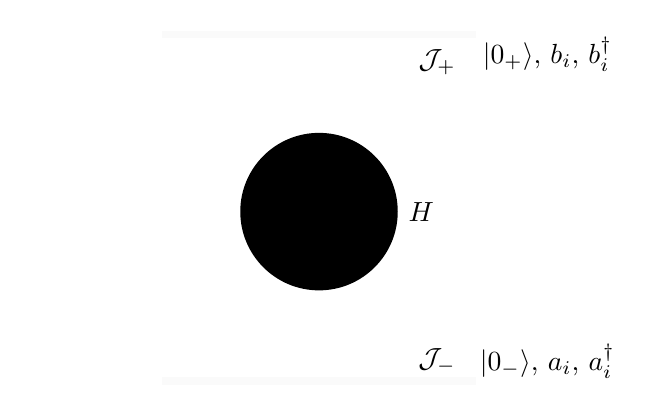
\begin{tikzpicture}
      \path (-3.7,0) -- (0,0);



      \fill[color=white!98!black] (-2,2.2) rectangle +(4,0.1);

      \node at (1.5,1.9) {$\mathcal{J}_{ + }$};

      \node[align=left] at (2.9,2) {$| 0_{ + } \rangle$, $b_{ i }$,
        $b_{ i }^{ \dagger }$};



      \fill[color=black] (0,0) circle [radius=1];

      \node at (1.3,0) {$H$};


      \fill[color=white!98!black] (-2,-2.2) rectangle +(4,0.1);

      \node at (1.5,-1.9) {$\mathcal{J}_{ - }$};

      \node[align=left] at (2.9,-1.9) {$| 0_{ - } \rangle$, $a_{ i }$,
        $a_{ i }^{ \dagger }$};
    \end{tikzpicture}

    \caption{Ilustracja podejścia Hawkinga}

  \end{figure}
  % #############



  Ilość cząstek wypromieniowanych przez czarną dziurę to „oczywiście”
  \begin{equation}
    \label{eq:Promieniowanie-Hawkinga-12}
    N = \langle 0_{ - } | \sum_{ i } b_{ i }^{ \dagger } b_{ i } | 0_{ - } \rangle
  \end{equation}

\end{frame}
% ##################





% ##################
\begin{frame}{Szkic obliczeń}
  \frametitle{Jak obliczyć $N$?}


  \begin{align}
    \label{eq:Promieniowanie-Hawkinga-13}
    &N = \sum_{ i } N_{ i } =
      \sum_{ i } \langle 0_{ - } | b_{ i }^{ \dagger } b_{ i } | 0_{ - } \rangle \\
    &\widehat{ b }_{ i } =
      \sum_{ j } ( \bar{ \alpha }_{ i j }\, \widehat{ a }_{ j }
      - \bar{ \beta }_{ i j }\, \widehat{ a }^{ \dagger }_{ j } ), \\
    &N_{ i } =
      \langle 0 | \widehat{ b }^{ \dagger }_{ i } \widehat{ b }_{ i } | 0 \rangle =
      \sum_{ j } | \beta_{ i j } |^{ 2 }.
  \end{align}
  Uwzględniając rozkład na mody sferyczne, w sposób dość zawiły
  definiujemy za pomocą $\alpha_{ ij }$ i~$\beta_{ ij }$ współczynnik
  $\Gamma_{ jnlm }$.

  Hawking policzył, że ilość wyemitowanych cząstek w modzie $jnlm$ dla
  czarnej dziury Schwarzschilda spełnia rozkład
  \begin{equation}
    \label{eq:Promieniowanie-Hawkinga-14}
    N_{ jnlm } =
    \Gamma_{ jnlm } \frac{ 1 }{ e^{ \frac{ 2\pi }{ \kappa } \omega } - 1 }.
  \end{equation}

\end{frame}
% ##################





% ##################
\begin{frame}{Szkic obliczeń}
  \frametitle{Wynik}

  \begin{equation}
    \label{eq:Promieniowanie-Hawkinga-15}
    N_{ jnlm } =
    \Gamma_{ jnlm } \frac{ 1 }{ e^{ \frac{ 2\pi }{ \kappa } \omega } - 1 }.
  \end{equation}

  Jest on taki jak dla promieniowania termicznego ciała dla którego
  zachodzi $E / k_{ B } T = 2\pi \omega / \kappa$. Wracając do stałych
  fizycznych i~kładąc $E = \hbar \omega$ dostajemy
  \begin{equation}
    \label{eq:Promieniowanie-Hawkinga-15}
    T = \frac{ \hbar \kappa }{ 2\pi k_{ \mathrm{B} } } =
    \frac{ \hbar }{ 2\pi c } A \approx
    10^{ -6 } \left( \frac{ M_{ \odot } }{ M_{ BH } } \right)
    {}^{ \circ } \mathrm{K},
  \end{equation}
  gdzie $A$ to powierzchnia czarnej dziury. Według Hawkinga podobny
  wyniki zachodzi dla pola elektromagnetycznego i~zlinearyzowanej
  grawitacji.

\end{frame}
% ##################










% ######################################
\section{Lokalna analiza pól kwantowych na zakrzywionych
  czasoprzestrzeniach}
% ######################################



% ##################
\begin{frame}
  \frametitle{Wątpliwości jakie pozostawiła praca Hawkinga}


  \begin{itemize}
    \RaggedRight

  \item Obliczenia wykorzystywały przybliżenie optyki geometrycznej,
    jego prawomocność nie jest wcale pewna.

  \item Użyta została statyczna metryka Schwarzschilda, a tylko
    dynamiczny proces kolapsu powinien powodować kreację cząstek. Nie
    potrafiłem zrozumieć argumentów z pracy Hawkinga czemu można użyć
    tej metryki.

  \item Konieczne jest narzucenie warunków brzegowych na rodzinę
    funkcji zespolonych, które opisują ich zachowanie na istniejącym
    zawsze i od zawsze brzegu czarnej dziury.

  \item Problem nierównoważności przestrzeni Hilberta o różnych
    stanach próżni wymagał dalszej analizy.

  \end{itemize}


  Przedstawię teraz pewną próbę doprecyzowania tej teorii podjętą w~ramach
  algebraicznej kwantowej teorii pola z~ery przedradzikowskiej,
  czyli przed 1996 rokiem.

\end{frame}
% ##################





% ##################
\begin{frame}
  \frametitle{Zasady lokalnej sensowności i stabilności}


  Rolą tej \textbf{zasada lokalnej sensowności} (ang. \textit{principle
    of local definiteness}, tłumaczenie autorskie) i~podanej
  wspomnianej dalej \textbf{zasady lokalnej stabilności} jest
  wykluczenie z rozważań pewnych teorii pola, które uważamy za
  nierealistyczne. W~czasoprzestrzeni Minkowskiego podobne teorie są
  wykluczane przez warunek zgodności z~grupą Poincar\'{e}go.

  Rozważmy mały obszar czasoprzestrzeni ściągalny do punktu
  $\Ocal$.





  % #############
  \begin{figure}[h]

    \begin{tikzpicture}[scale=0.8]
      % \path (-3.7,0) -- (0,0);

      \fill[color=gray,opacity=0.9,rounded corners=3pt] (-2,0.5) --
      (-1,1.5) -- (0.5,0.8) -- (2.5,0.6) -- (0.8,-0.8) -- (0.2,-1.5) --
      (-1,-1.2) -- cycle;


      \draw[dashed,color=black!90] (0,0) -- (1.7,0.3);

      \draw[dashed,color=black!90] (0,0) -- (0.1,-1);

      \draw[dashed,color=black!90] (0,0) -- (-1.5,0.5);

      \draw[dashed,color=black!90] (0,0) -- (-0.9,1.1);



      \fill[color=jOrange] (0,0) circle [radius=0.1];
    \end{tikzpicture}

    \caption{Obszar ściągalny do punktu}

  \end{figure}
  % #############

\end{frame}
% ##################





% ##################
\begin{frame}
  \frametitle{Zasady lokalnej sensowności i stabilności}


  Ponieważ reguły nadwyboru mają charakter globalny, jak zasada
  zachowania ładunku elektrycznego, albo topologiczny, czyli nie mogą
  odgrywać roli w~odpowiednio małym ściągalnym do punktu obszarze,
  dlatego postulujemy następującą zasadę.

  \textbf{Zasada lokalnej sensowności.} Zbiór stanów pola kwantowego
  mierzalnych w~odpowiednio małym ściągalnym obszarze $\Ocal$
  nie dopuszcza żadnych reguł nadwyboru.

  \textbf{Zasada lokalnej stabilności} z~grubsza rzecz biorąc mówi,
  że~to co możemy uznać za lokalnie najbardziej symetrycznych stan jest
  też lokalnym stanem próżni. Dokładne wyjaśnienie tego zagadnienia
  przekracza jednak ramy tego seminarium.

\end{frame}
% ##################





% ##################
\begin{frame}
  \frametitle{Zasady lokalnej stabilności a fizyka}


  W 1984 roku Rudolf Haag, Heide Narnhofer i~Ulrich Stein pokazali, że
  wewnątrz tego podejścia dla pola kwantowego dopuszczalne są różne
  stany $| \psi \rangle$ opisujące pole w równowadze termodynamicznej,
  ale tylko te o temperaturze $T = \frac{ \hbar }{ 2\pi c } A$
  spełniają warunek lokalnej stabilności na horyzoncie czarnej dziury
  \cite{FredenhagenHaagDerivationOfHawkingRadiation1990}.

  W dalszym ciągu wygodnie będzie zapisać warunek lokalnej stabilności
  za pomocą funkcji dwupunktowej.

  Funkcję dwupunktową pola $\widehat{ \phi }( x )$ dla stanu $\psi$
  definiujemy funkcję dwupunktową
  $W^{ ( 2 ) }_{ \psi }( x_{ 1 }, x_{ 2 } )$ wzorem
  \begin{equation}
    \label{eq:Promieniowanie-Hawkinga-16}
    W^{ ( 2 ) }_{ \psi }( x_{ 1 }, x_{ 2 } ) =
    \langle \psi | \widehat{ \phi }( x_{ 1 } ) \widehat{ \phi }( x_{ 2 } ) | \psi \rangle.
  \end{equation}
  Już w czasoprzestrzeni Minkowskiego
  $W^{ ( 2 ) }_{ \psi }( x_{ 1 }, x_{ 1 } )$ jest czymś w rodzaju
  $\delta( x_{ 1 } - x_{ 1 } ) = \delta( 0 )$, czyli by zacytować
  naszego kolegę „To jest jakiś nonsens”. Dlatego spodziewamy się, że
  na małych odległościach $W^{ ( 2 ) }_{ \psi }( x_{ 1 }, x_{ d } )$
  będzie osobliwą funkcją.

\end{frame}
% ##################





% ##################
\begin{frame}
  \frametitle{Zasady lokalnej stabilności a fizyka}

  \vspace{-1em}


  \begin{equation}
    \label{eq:Promieniowanie-Hawkinga-17}
    W^{ ( 2 ) }_{ \psi }( x_{ 1 }, x_{ 2 } ) =
    \langle \psi | \widehat{ \phi }( x_{ 1 } ) \widehat{ \phi }( x_{ 2 } ) | \psi \rangle
  \end{equation}

  Warunek lokalnej stabilności możemy przetłumaczyć na postulat, że
  dla stanu $| \psi \rangle$ jego funkcja dwupunktowa
  $W^{ ( 2 ) }_{ \psi }( x_{ 1 }, x_{ 1 } )$ może być zapisana w~następujący sposób:
  \begin{equation}
    \label{eq:Promieniowanie-Hawkinga-18}
    W^{ ( 2 ) }_{ \psi }( x_{ 1 }, x_{ 1 } ) =
    \frac{ 1 }{ ( 2 \pi )^{ 2 } } \frac{ 1 }{ \sigma( x_{ 1 }, x_{ 2 } ) }
    + w_{ \psi }( x_{ 1 }, x_{ 2 } ).
  \end{equation}
  Symbol $\sigma( x_{ 1 }, x_{ 2 } )$ oznacza kwadrat odległości
  geodezyjnej między $x_{ 1 }$, $x_{ 2 }$, zaś $w( x_{ 1 }, x_{ 2 } )$
  jest odpowiednio gładka i~znika na stożku świetlnym.

  Ścisłe sformułowanie tych warunków jakie ma spełniać rozkład
  \eqref{eq:10} jest czasochłonne i nie wnosi wiele do tego
  seminarium. To co jest naprawdę ważne, to to że warunek lokalnej
  stabilności wyrażony tym równaniem wiąże zachowanie pól kwantowych
  ze strukturą geodezyjną czasoprzestrzeni.

\end{frame}
% ##################










% ######################################
\section{Promieniowanie Hawkinga a~kolaps sferycznie symetrycznej
  gwiazdy}
% ######################################



% ##################
\begin{frame}
  \frametitle{Kolapsująca gwiazda}


  Przedstawione tu wyniki pochodzą z pracy Rudolfa Haaga i Klausa
  Fredenhagena \textit{On the Derivation of Hawking Radiation Associated
    with the Formation of a Black Hole} z 1990 roku. Zrozumieli oni,
  że jeśli uwzględniamy w równaniach Einsteina tylko sferycznie
  symetryczną kolapsującą gwiazdę i interesuje nas rezultat jaki
  zmierzy obserwator który wraz ze swoim detektorem przystąpi do badań
  promieniowania czarnej dziury na długo po jej utworzeniu się, to
  wystarczy nam znajomość metryki na zewnątrz zapadającej się gwiazdy.
  Uratuje nas od tego twierdzenie Birkhoffa.

  Twierdzenie to stwierdza, że jeśli jedynym obiektem którego wpływa
  na metrykę uwzględniamy w równaniach Einsteina jest ciało sferycznie
  symetrycznych, to na jego zewnętrze metryka jest dana przez
  rozwiązanie Schwarzschilda.
  \begin{equation}
    \label{eq:Promieniowanie-Hawkinga-19}
    ds^{ 2 } =
    -\left( 1 - \frac{ r_{ 0 } }{ r } \right) dt^{ 2 }
    + \left( 1 - \frac{ r_{ 0 } }{ r } \right)^{ -1 } dr^{ 2 }
    + r^{ 2 } ( d \theta^{ 2 } + ( \sin\theta )^{ 2 } \, d\phi^{ 2 } ).
  \end{equation}

\end{frame}
% ##################





% ##################
\begin{frame}
  \frametitle{Kolapsująca gwiazda}

  \vspace{-1em}


  \begin{equation}
    \label{eq:Promieniowanie-Hawkinga-20}
    ds^{ 2 } =
    -\left(1 - \frac{ r_{ 0 } }{ r } \right) dt^{ 2 }
    + \left(1 - \frac{ r_{ 0 } }{ r } \right)^{ -1 } dr^{ 2 }
    + r^{ 2 } ( d \theta^{ 2 } + ( \sin \theta )^{ 2 } d\phi^{ 2 } ).
  \end{equation}
  Promień Schwarzschilda oznaczam dla wygody $r_{ 0 }$.

  W czasoprzestrzeni wprowadzamy standardowe zmienne Schwarzchilda
  $t$, $r$, $\theta$, $\varphi$ wszędzie gdzie mają sens. Dodatkowo wprowadzamy
  współrzędną czasową $\tau$ która jest nieosobliwa na horyzoncie
  i~zbliża~się $t$ dla $r >> r_{ 0 }$.

  Niech $r_{ S }( \tau )$ opisuje nam promień gwiazdy w chwili $\tau$.
  Mam dużą swobodę wyboru postaci funkcji $r_{ S }( \tau )$, ważne dla
  nas jest tylko to by kolaps był zawsze sferycznie symetryczny.

  Dla wygody przyjmijmy, że $r_{ s }( 0 ) = r_{ 0 }$. Oznacza to, że w
  chwili $\tau = 0$ gwiazda przecina swój promień Schwarzschilda i~formuje
  czarną dziurę.

\end{frame}
% ##################





% ##################
\begin{frame}
  \frametitle{Kolapsująca gwiazda}


  Oznaczmy przez $A$ obszar w czasoprzestrzeni na zewnątrz
  kolapsującej gwiazdy, jest on określony dwoma równaniami
  \begin{equation}
    \label{eq:Promieniowanie-Hawkinga-21}
    r > r_{ 0 }, \quad
    r > r_{ S }( \tau ).
  \end{equation}
  W tym obszarze możemy zdefiniować nasze współrzędne jako
  \begin{subequations}
    \begin{align}
      \label{eq:Promieniowanie-Hawkinga-22-A}
      &r^{ * } = r + r_{ 0 } \ln( \frac{ r }{ r_{ 0 } } - 1 ), \\
      \label{eq:Promieniowanie-Hawkinga-22-B}
      &u = t + r^{ * }, \\
      \label{eq:Promieniowanie-Hawkinga-22-C}
      &v = t - r^{ * }, \\
      \label{eq:Promieniowanie-Hawkinga-22-D}
      &\tau = v - r = t + r^{ * } - r.
    \end{align}
  \end{subequations}

  Moją one porządne przez nas własności.

\end{frame}
% ##################





% ##################
\begin{frame}
  \frametitle{Detektor pola}


  Znowu będziemy analizować pole skalarne $\widehat{\phi}( x )$
  spełniające dobrze znane nam równanie
  \begin{equation}
    \label{eq:Promieniowanie-Hawkinga-23}
    g^{ \mu \nu }( x ) \nabla_{ \mu } \nabla_{ \nu } \widehat{\phi}( x ) = 0.
  \end{equation}
  Co to jest detektor pola? Jest to urządzenie które ustawia nasz
  obserwator by w skończonym obszarze (zbudowanie nieskończonego
  detektora napotyka pewne trudności techniczne) i w skończonym czasie
  (problemy z budżetem) zliczyć ilość cząstek.

  Niech $\mathcal{O}_{ T }$ będzie ograniczonym (względnie zwartym)
  obszarem przestrzeni daleko od kolapsującej gwiazdy. Jeśli pole
  kwantowe jest w stanie $| \psi \rangle$ to możemy zdefiniować detektor jako
  \begin{subequations}
    \begin{align}
      \label{eq:Promieniowanie-Hawkinga-24-A}
      &N_{ \psi }( T ) = \langle \psi | Q^{ * }( T ) Q( T )  | \psi \rangle, \\
      \label{eq:Promieniowanie-Hawkinga-24-B}
      &Q( T ) = \int_{ \Ocal_{ T } } \widehat{\phi}( x_{ 1 } )
        h( T - t_{ 1 }, \underline{x} ) \sqrt{ | g( x_{ 1 } ) | }
        d^{ 4 }x_{ 1 }
    \end{align}
  \end{subequations}

\end{frame}
% ##################





% ##################
\begin{frame}
  \frametitle{Detektor pola}

  \vspace{-2em}


  \begin{subequations}
    \begin{align}
      \label{eq:Promieniowanie-Hawkinga-25-A}
      &N_{ \psi }( T ) = \langle \psi | Q^{ * }( T ) Q( T )  | \psi \rangle, \\
      \label{eq:Promieniowanie-Hawkinga-25-B}
      &Q( T ) =
        \int_{ \Ocal_{ T } } \widehat{\phi}( x_{ 1 } )
        h( T - t_{ 1 }, \underline{x_{ 1 }} )
        \sqrt{ | g( x_{ 1 } ) | } \, d^{ 4 }x_{ 1 }
    \end{align}
  \end{subequations}
  Funkcja $h( T - t, \underline{x} )$ jest tak dobrany by jej nośnik
  zawierała się w zbiorze $\mathcal{O}_{ T }$ i by znikała dla
  $t \notin [ T - \Delta t, T + \Delta t]$, $\Delta t$ jest ustalone.
  Używam takiej notacji by przejście graniczne $T \to +\infty$ było
  łatwiejsze do zobrazowania. Dla wygody nie będę już pisał indeksu
  $\psi$.

  \vspace{-1em}


  \begin{equation}
    \label{eq:Promieniowanie-Hawkinga-26}
    \begin{split}
      &N( T ) = \langle \psi | Q^{ * }( T ) Q( T ) | \psi \rangle = \\
      &= \int_{ \Ocal_{ T } } \int_{ \Ocal_{ T } } \langle \psi | \widehat{\phi}( x_{ 1 } )
        \widehat{\phi}( x_{ 2 } ) | \psi \rangle
        h( T - t_{ 1 }, \underline{x_{ 1 }} ) h( T - t_{ 2 },
        \underline{x_{ 1 }} ) \sqrt{ | g( x_{ 1 } ) | } \, \times \\
      &\times \, \sqrt{ | g( x_{ 2 } ) | } \, d^{ 4 }x_{ 1 }\, d^{ 4 }x_{ 2 } =
        \int_{ \Ocal_{ T } } \int_{ \Ocal_{ T } } W^{ ( 2 ) }( x_{ 1 }, x_{ 2 } )
      h( T - t_{ 1 }, \underline{x_{ 1 }} ) \, \times \\
      &\times \, h( T - t_{ 2 }, \underline{x_{ 1 }} )
        \sqrt{ | g( x_{ 1 } ) | } \sqrt{ | g( x_{ 2 } ) | } \,
        d^{ 4 }x_{ 1 }\, d^{ 4 }x_{ 2 }
    \end{split}
  \end{equation}

\end{frame}
% ##################





% ##################
\begin{frame}
  \frametitle{Teraz będzie sztuczka}


  Widzimy, że $N( T )$ zależy od funkcji dwupunktowej
  $W^{ ( 2 ) }( x_{ 1 }, x_{ 2 } )$.

  Teraz wykonany bardzo niebanalny krok. Ponieważ
  $\widehat{\phi}( x )$ spełnia równanie pola, więc
  $W^{ ( 2 ) }( x_{ 1 }, x_{ 2 } )$ spełnia równanie pola osobno w
  każdym argumencie. (Czy to widać?)

  Dzięki temu \textit{istnieje} taka funkcja zespolona $f^{ T }( x )$
  spełniająca równanie pola taka, że
  \begin{equation}
    \label{eq:Promieniowanie-Hawkinga-27}
    \begin{split}
      &\int_{ \Ocal_{ T } } W^{ ( 2 ) }( x_{ 1 }, x_{ 2 } )
        h( T - t_{ 1 }, \underline{x_{ 1 }} )
        \sqrt{ | g( x_{ 1 } ) | }\, d^{ 4 }x_{ 1 } = \\
      &= \int_{ \Sigma_{ 1 } } W^{ ( 2 ) }( x_{ 1 }, x_{ 2 } )
        \overleftrightarrow{ \frac{ \partial }{ \partial x_{ 1 }^{ \mu } } }
        f^{ T }( x_{ 1 } ) d\sigma_{ 1 }^{ \mu }.
    \end{split}
  \end{equation}
  $\Sigma_{ 1 }$ to dowolna powierzchnia Cauchy’ego, a~$d\sigma_{ 1 }^{ \mu }$ to
  element powierzchni.

\end{frame}
% ##################




% ##################
\begin{frame}
  \frametitle{Teraz będzie sztuczka}


  W szczególności za powierzchnię Cauchy’ego możemy wybrać
  powierzchnię daną równaniem $\tau = 0$, oznaczmy ją $\Sigma$. Mamy
  więc wspaniałą zależność.
  \begin{equation}
    \label{eq:Promieniowanie-Hawkinga-28}
    \begin{split}
      &N( T ) =
        \int_{ \Sigma } \int_{ \Sigma } W^{ ( 2 ) }( x_{ 1 }, x_{ 2 } )
        \overleftrightarrow{ \frac{ \partial }{ \partial x_{ 1 }^{ \mu } } }
        f^{ T }( x_{ 1 } ) \overleftrightarrow{ \frac{ \partial }{ \partial x_{ 2 }^{ \mu } } }
        f^{ T }( x_{ 2 } ) d\sigma_{ 1 }^{ \mu } d\sigma_{ 2 }^{ \mu }
    \end{split}
  \end{equation}

  Co więcej dla $\tau \geq 0$ przestrzenny nośnik $f^{ T }( x )$ leży
  cały w obszarze $A$, czyli poza czarną dziurą. Ma to sens z
  fizycznego punktu widzenia, gdyby jego część znajdowała się w
  czarnej dziurze, to sygnał od niej nigdy nie dotarłby do detektora.
  A to oznacza, że do równania na tę wchodzi tylko metryka
  Schwarzschilda!

\end{frame}
% ##################






% ##################
\begin{frame}
  \frametitle{Teraz będą rachunki}


  Zapisujemy funkcję $f^{ T }( x )$ we współrzędnych $t$, $r^{ * }$,
  $\theta$, $\varphi$ i rozkładamy na mody „sferyczne”.
  \begin{equation}
    \label{eq:Promieniowanie-Hawkinga-29}
    f^{ T }( t, r^{ * }, \theta, \varphi ) =
    \frac{ 1 }{ r }
    \sum_{ l,\, } f^{ T }_{ lm }( t, r^{ * } ) Y^{ l }_{ m }( \theta, \varphi )
  \end{equation}

  Wstawiając tą postać do równania „falowego” dostajemy.
  \begin{align}
    \label{eq:Promieniowanie-Hawkinga-30-A}
    &( \frac{ \partial^{ 2 } }{ \partial t^{ 2 } } - \frac{ \partial^{ 2 } }{ \partial r^{ *\, 2 } }
      + V_{ l }( r ) ) f^{ T }_{ lm }( t, r^{ * } ) = 0 \\
    \label{eq:Promieniowanie-Hawkinga-30-B}
    &V_{ l }( r ) =
      ( 1 - \frac{ r_{ 0 } }{ r } ) ( \frac{ l ( l + 1 ) }{ r }
      + \frac{ r_{ 0 } }{ r^{ 3 } })
  \end{align}
  Państwo lepiej niż ja rozumieją sens tego równania.

  Haag i Fredenhagen rozwiązali je korzystając z transformaty
  Fouriera, transformaty Laplace, sferycznych funkcji Hankela i kilku
  innych technik. Nawet nie próbujmy teraz powtarzać ich rachunków.

\end{frame}
% ##################





% ##################
\begin{frame}
  \frametitle{Teraz będą rachunki}


  W dalszym ciągu będzie ważne to, że musimy rozwiązać problem
  rozpraszania na potencjale $V_{ l }( r )$ i wyznaczyć jego
  współczynniki transmisji $D_{ l }( \omega )$.

  Dla dużych wartość $T$ możemy zapisać
  $f^{ T }_{ l m }( t, r^{ * } )$ jako sumę trzech członów.
  \begin{equation}
    \label{eq:Promieniowanie-Hawkinga-31}
    f^{ T }_{ l m }( t, r^{ * } ) =
    f^{ T }_{ +,\, l m }( t, r^{ * } ) + f^{ T }_{ -,\, l m }( t, r^{ * } )
    + \Delta_{ lm }^{ T }( t, r^{ * } )
  \end{equation}

  Człon $\Delta_{ lm }^{ T }( t, r^{ * } )$ opisuje fale które przy
  $T \to +\infty$ „rozpływają się” po całej przestrzeni i tym samy nie
  dają wkładu do $N( T )$. Człon $f_{ +,\, lm }^{ T }( t, r^{ * } )$
  opisuje pakiet falowy który w tej samej granic co poprzednio ucieka
  do nieskończoności, więc też nie daje wkładu do $N( T )$.

  Człon $f_{ -,\, lm }^{ T }( t, r^{ * } )$ opisuje pakiet falowy,
  który „biegnie” w kierunki $r_{ 0 }$, zawsze jednak pozostaje w
  obszarze $r > r_{ 0 }$.

\end{frame}
% ##################





% ##################
\begin{frame}
  \frametitle{Teraz będą rachunki}


  Możemy zapisać
  \begin{equation}
    \label{eq:Promieniowanie-Hawkinga-32}
    f^{ T }_{ -,\, l m }( t, r^{ * } ) =
    \psi\big( \xi( \tau, r ) / \exp( -T / 2 r_{ 0 } ) \big), \quad
    \xi( \tau, r ) =
    \frac{ r - r_{ 0 } }{ r_{ 0 } } e^{ -\tau / 2 r_{ 0 } }
  \end{equation}
  O funkcji $\psi( y )$ potrzebujemy wiedzieć tylko, że
  $\psi( 0 ) = 0$ i znika w~nieskończoności. Dla $T \to +\infty$ dąży
  do $0$ wszędzie poza kurczącym się otoczeniem punktu $r_{ 0 }$.

  \begin{equation}
    \label{eq:Promieniowanie-Hawkinga-33}
    \begin{split}
      &N( T ) =
        \int_{ \Sigma } \int_{ \Sigma } W^{ ( 2 ) }( x_{ 1 }, x_{ 2 } )
        \overleftrightarrow{ \frac{ \partial }{ \partial x_{ 1 }^{ \mu } } }
        f^{ T }( x_{ 1 } ) \overleftrightarrow{ \frac{ \partial }{ \partial x_{ 2 }^{ \mu } } }
        f^{ T }( x_{ 2 } ) d\sigma_{ 1 }^{ \mu } d\sigma_{ 2 }^{ \mu }
    \end{split}
  \end{equation}

  W takiej sytuacji z~powyższej całki w granicy $T \to +\infty$
  przeżywa tylko człon w którym $f^{ T }_{ -,\, l m }( t, r^{ * } )$
  jest mnożone przez człon osobliwy $1 / \sigma( x_{ 1 }, x_{ 2 } )$ z
  funkcji dwupunktowej. Przypomnijmy, że jest on równoważny lokalnej
  stabilności pola.

\end{frame}
% ##################





% ##################
\begin{frame}
  \frametitle{Wynik}


  \begin{equation}
    \label{eq:Promieniowanie-Hawkinga-34}
    \lim_{ T \to +\infty } N( T ) =
    C \sum_{ l,\, m }
    \int\limits_{ -\infty }^{ +\infty } d\omega \, \abs{ D_{ l }( \omega ) }^{ 2 }
    \frac{ \abs{ \widetilde{h}_{ lm }( \omega, -\omega ) } }{ \omega ( 1 - e^{ -\beta \omega } ) }
  \end{equation}

  $\beta = 4 \pi r_{ 0 }$, $\widetilde{h}_{ lm }( \omega, -\omega )$
  opisuje „rozdzielczość” używanego detektora, $D_{ l }( \omega )$ to
  współczynnik transmisji przez potencjał $V_{ l }( \omega )$.

\end{frame}
% ##################





% ##################
\begin{frame}
  \frametitle{Wnioski}


  1) Promieniowanie Hawkinga zostaje wytworzone w krótkiej chwili
  czasu, mierzonego w układzie zapadającej się gwiazdy, gdy promień
  gwizdy przekracza jej promień Schwarzchilda. To, że można je
  obserwować przez bardzo długi czas, to wynik dylatacji czasu.

  2) Obliczenia przewidują nieskończoną ilość energii wytworzoną
  w~chwili kolapsu. Ten nierealistyczny wynik wynika zapewne z tego,
  że~nie uwzględniliśmy działania wpływu energii pola na metrykę.

  3) Nawet dla swobodne pola należy uwzględnić to, że~część
  promieniowania przechodzi przez $r_{ 0 }$ tuż przez kolapsem.
  W~przypadku oddziałujących modeli pól, choćby chromodynamiki, sytuacja
  nie wydaje się upraszczać.

\end{frame}
% ##################









% ######################################
\appendix
% ######################################





% ##################
\EndingSlide{Dziękuję! Pytania?}
% ##################










% ######################################
\section{Szkic obliczeń Hawkinga dla czarnej dziury Schwarzschilda}
% ######################################



% ##################
\begin{frame}
  \frametitle{Co można zrobić?}


  \begin{itemize}

  \item[1.] Poddać~się i~porzucić badanie tego problemu.

  \item[2.] Dojść do~wniosku, że~na zakrzywionej czasoprzestrzeni
    pojęcie cząstki nie ma sensu (z~punktu widzenia fizyki
    teoretycznej).

  \item[3.] Rozpatrzeć przypadek, gdzie coś da~się powiedzieć.

  \end{itemize}

  Wybieramy przypadek numer 3. \\

  Jeżeli czasoprzestrzeń $M$ zawiera obszar który jest płaski (lub
  asymptotycznie płaski), wtedy istnieje w~nim kanoniczny czas
  i~używają go możemy zdefiniować rodzinę rozwiązań równań pola
  skalarnego o~dodatnich częstościach. Niemniej jeśli mamy dwa takie
  obszary nie możemy zwykle powiązać czasu w~jednym obszarze z~czasem
  w~drugim. Co~to oznacza?

\end{frame}
% ##################





% ##################
\begin{frame}
  \frametitle{Efekt Hawkinga dla~czarnej dziury Schwarzschilda}

  Aby obliczyć ilość „cząstek wypromieniowanych przez czarną dziurę”
  \begin{equation}
    \label{eq:Promieniowanie-Hawkinga-35}
    N =
    \langle 0_{ - } | \sum_{ i } \widehat{ b }_{ i }^{ \dagger } \widehat{ b }_{ i } \,
    | 0_{ - } \rangle,
  \end{equation}
  Hawking wykonał całkiem pomysłowy i~dość żmudny rachunek. W~dalszym
  ciągu naszkicuję jak on~wyglądał oraz do~jakich wniosków prowadzi.

  Metrykę dla czarnej dziura Schwarzschilda można odczytać z
  poniższego, dobrze znanego wzoru.
  \begin{equation}
    \label{eq:Promieniowanie-Hawkinga-36}
    ds^{ 2 } =
    -\left(1 - \frac{ 2M }{ r } \right) dt^{ 2 }
    + \left(1 - \frac{ 2M }{ r } \right)^{ -1 } dr^{ 2 }
    + r^{ 2 } ( d \theta^{ 2 } + ( \sin \theta )^{ 2 } d\phi^{ 2 } ).
  \end{equation}
  Przyjęliśmy „naturalny układ jednostek” $c = 1$, $G = 1$,
  $\hbar = 1$, $k_{ \textrm{B} } = 1$.

\end{frame}
% ##################





% ##################
\begin{frame}
  \frametitle{Warunki ortogonalności}


  Będziemy rozpatrywali rodziny rozwiązań równania pola skalarnego,
  \begin{equation}
    \label{eq:Promieniowanie-Hawkinga-37}
    g^{ \mu \nu }( x ) \nabla_{ \mu } \nabla_{ \nu } \widehat{ \phi }( x ) = 0.
  \end{equation}
  spełniające warunek:
  \begin{equation}
    \label{eq:Promieniowanie-Hawkinga-38}
    \frac{ 1 }{ 2 } i\int_{ S } ( \, f_{ i }( x )
    \nabla_{ a }\bar{ f }_{ j }( x ) - f_{ j }( x )
    \nabla_{ a } \bar{ f }_{ i }( x ) )\, d\sigma_{ a }
    = \delta_{ i j },
  \end{equation}
  gdzie $S$ to~pewna wybrana powierzchnia.

  W~czasoprzestrzeni Schwarzschilda~są trzy ważne dla tego problemu
  powierzchnie.
  \begin{itemize}

  \item[1.] Horyzont czarnej dziury $H$.

  \item[2.] Nieskończona przeszłość świetlna $\Jcal_{ - }$.

  \item[3.] Nieskończona przyszłość świetlna $\Jcal_{ + }$.

  \end{itemize}

\end{frame}
% ##################





% ##################
\begin{frame}
  \frametitle{To nie jest diagram Penrose’a!}


  % #############
  \begin{figure}[h]

    \centering

    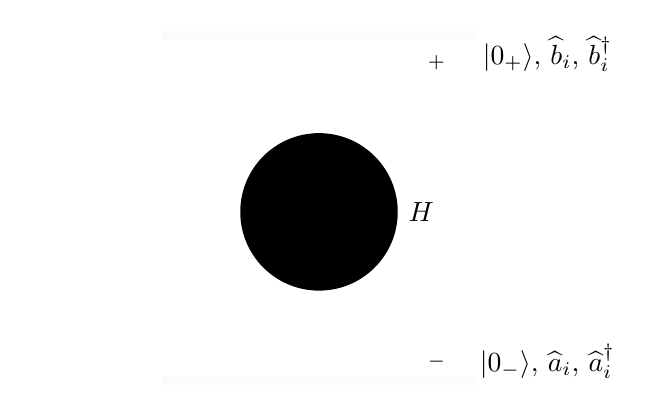
\begin{tikzpicture}
      \path (-3.7,0) -- (0,0);



      \fill[color=white!98!black] (-2,2.2) rectangle +(4,0.1);

      \node at (1.5,1.9) {$\Jcal_{ + }$};

      \node[align=left] at (2.9,2) {$| 0_{ + } \rangle$,
        $\widehat{b}_{ i }$, $\widehat{b}_{ i }^{ \dagger }$};



      \fill[color=black] (0,0) circle [radius=1];

      \node at (1.3,0) {$H$};


      \fill[color=white!98!black] (-2,-2.2) rectangle +(4,0.1);

      \node at (1.5,-1.9) {$\Jcal_{ - }$};

      \node[align=left] at (2.9,-1.9) {$| 0_{ - } \rangle$,
        $\widehat{a}_{ i }$, $\widehat{a}_{ i }^{ \dagger }$};

    \end{tikzpicture}

    \caption{Interesujące nas powierzchnie}

  \end{figure}
  % #############

\end{frame}
% ##################





% ##################
\begin{frame}
  \frametitle{Ważne rodziny funkcji}


  \begin{itemize}

  \item Przez $f_{ i }( x )$ oznaczamy zupełny układ rozwiązań
    równania pola $\widehat{ \phi }( x )$, ortogonalnych względem
    całki po~$\Jcal_{ - }$. Przedstawiają cząstki przylatujące
    z~nieskończonej przeszłości czasowej.

  \item $p_{ i }( x )$~są ortogonalne względem całki
    na~$\Jcal_{ + }$ i~znikają wraz z~pierwszymi pochodnymi
    na~$H$. Przestawiają cząstki wylatujące z~czarnej dziury
    i~zmierzające do~nieskończonej przyszłość czasowej.

  \item $q_{ i }( x )$~są ortogonalne na~$H$ i~znikają
    na~$\Jcal_{ + }$. Przedstawia cząstki „złapane” przez czarna
    dziurę.

  \end{itemize}

\end{frame}
% ##################





% ##################
\begin{frame}
  \frametitle{Efekt Hawkinga dla~czarnej dziury Schwarzschilda}


  Pole $\widehat{ \phi }( x )$ jest określone w~całej czasoprzestrzeni,
  jeśli zadana jest jego wartość, wraz z~pierwszymi pochodnymi
  na~$\Jcal_{ - }$, lub jednocześnie na~$H$ i~$\Jcal_{ + }$. Możliwe są
  więc dwa następujące jego rozkłady na~mody normalne:
  \begin{equation}
    \label{eq:Promieniowanie-Hawkinga-39}
    \widehat{ \phi }( x )
    = \sum_{ i } ( \, f_{ i }( x ) \, \widehat{ a }_{ f,\, i }
    + \bar{ f }_{ i }( x ) \, \widehat{ a }^{ \dagger }_{ f,\, i } ),
  \end{equation}
  oraz
  \begin{equation}
    \label{eq:Promieniowanie-Hawkinga-40}
    \widehat{ \phi }( x ) =
    \sum_{ i }( p_{ i }( x ) \, \widehat{ b }_{ p,\, i }
    + \bar{ p }_{ i }( x ) \, \widehat{ b }^{ \dagger }_{ p,\, i }
    + q_{ i }( x )\, \widehat{ c }_{ q,\, i }
    + \bar{ q }_{ i }( x ) \, \widehat{ c }^{ \dagger }_{ q,\, i } ).
  \end{equation}

  Chcemy policzyć cząstek zaobserwowanych w~$\Jcal_{ + }$, czyli
  \begin{equation}
    \label{eq:Promieniowanie-Hawkinga-41}
    N =
    \langle 0_{ - } | \sum_{ i } \widehat{ b }^{ \dagger }_{ p,\, i }
    \widehat{ b }_{ p,\, i } | 0_{ - } \rangle.
  \end{equation}

\end{frame}
% ##################





% ##################
\begin{frame}
  \frametitle{Efekt Hawkinga dla~czarnej dziury Schwarzschilda}


  Ponieważ wiemy jak $\widehat{ a }_{ f,\, i }^{ \dagger }$,
  $\widehat{ a }_{ f,\, i }$ działają na~$| 0_{ - } \rangle$, problem
  będzie rozwiązany, jeśli wyrazimy za~ich pomocą
  $\widehat{ b }_{ p,\, i }^{ \dagger }$, $\widehat{ b }_{ p,\, i }$.
  By~to zrobić, zauważmy, że~$p_{ i }( x )$ i~$q_{ i }( x )$, możemy
  znów rozłożyć na funkcje $f_{ i }( x )$:
  \begin{subequations}
    \begin{equation}
      \label{eq:Promieniowanie-Hawkinga-42-A}
      p_{ i }( x ) =
      \sum_{ j }( \alpha_{ i j } f_{ j }( x ) + \beta_{ i j } \bar{ f }_{ j }( x ) ),
    \end{equation}
    \begin{equation}
      \label{eq:Promieniowanie-Hawkinga-42-B}
      q_{ i }( x ) =
      \sum_{ j }( \gamma_{ i j } f_{ j }( x ) + \eta_{ i j } \bar{ f }_{ j }( x ) ).
    \end{equation}
  \end{subequations}
  Podstawiają to~dostajemy
  \begin{equation}
    \label{eq:Promieniowanie-Hawkinga-43}
    \widehat{ \phi }( x ) =
    \sum_{ i }( p_{ i }( x )\, \widehat{ b }_{ p,\, i }
    + \bar{ p }_{ i }( x )\, \widehat{ b }^{ \dagger }_{ p,\, i }
    + q_{ i }( x )\, \widehat{ c }_{ q,\, i }
    + \bar{ q }_{ i }( x )\, \widehat{ c }^{ \dagger }_{ q,\, i } ).
  \end{equation}

\end{frame}
% ##################





% ##################
\begin{frame}
  \frametitle{Rozkład „sferyczny”}


  We~współrzędnych „sferycznych” zupełny układ funkcji jest dany
  przez $f_{ \omega l m }( x )$, „numerowanych” ciągłym wskaźnikiem
  częstości $\omega$. Tym samym zmieniają~się też indeksy
  współczynników $\alpha_{ \omega l m\, \omega' l' m' }$ i~$\beta_{ \omega l m\, \omega' l' m' }$. Definiujemy
  \begin{equation}
    \label{eq:Promieniowanie-Hawkinga-44}
    p_{ \omega l m }( x ) =
    \int\limits_{ 0 }^{ +\infty } ( \alpha_{ \omega l m\, \omega' l m } \, f_{ \omega' l m }( x )
    + \beta_{ \omega l m\, \omega' l m } \, \bar{ f }_{ \omega' l m }( x ) ) \, d \omega'.
  \end{equation}

  Niech $p_{ \omega l m }^{ ( 1 ) }( x )$ oznacza rozwiązanie, które
  propaguje~się wstecz w czasie, rozprasza na~statycznej czarnej
  dziurze Schwarzchilda i~dociera na~$\Jcal^{ - }$ z~tą samą
  częstością~$\omega$. Dokonujemy rozkładu
  \begin{equation}
    \label{eq:Promieniowanie-Hawkinga-45}
    p_{ \omega l m }( x ) =
    p_{ \omega l m }^{ ( 1 ) }( x ) + p_{ \omega l m }^{ ( 2 ) }( x ).
  \end{equation}

\end{frame}
% ##################





% ##################
\begin{frame}
  \frametitle{Efekt Hawkinga dla~czarnej dziury Schwarzschilda}


  Analogicznie rozkładamy współczynniki
  \begin{subequations}
    \begin{align}
      \label{eq:Promieniowanie-Hawkinga-45-A}
      \alpha_{ \omega l m\, \omega' l m }
      &= \alpha_{ \omega l m\, \omega' l m }^{ ( 1 ) }
        + \alpha_{ \omega l m\, \omega' l m }^{ ( 2 ) }, \\
      \label{eq:HawkingPromieniowanie-45-B}
      \beta_{ \omega l m\, \omega' l m }
      &= \beta_{ \omega l m\, \omega' l m }^{ ( 1 ) }
        + \beta_{ \omega l m\, \omega' l m }^{ ( 2 ) }.
    \end{align}
  \end{subequations}


  Definiujemy nową rodzinę modów
  \begin{equation}
    \label{eq:HawkingPromieniowanie-46}
    p_{ j n l m }( x ) =
    \varepsilon^{ -\frac{ 1 }{ 2 } } \int\limits_{ j \varepsilon }^{ ( j + 1 ) \varepsilon }
    e^{ -2 \pi i\, \mathrm{n} \omega / \varepsilon } p_{ \omega l m }( x ) \, d \omega,
    \quad j = 0, 1, 2, \ldots
  \end{equation}
  gdzie $\varepsilon > 0$. Potrzebujemy jeszcze jednej wielkości
  \begin{equation}
    \label{eq:HawkingPromieniowanie-47}
    \Gamma_{ j n lm } =
    \int\limits_{ 0 }^{ +\infty }
    \left( \absOne{ \alpha_{ j n \omega' l m }^{ ( 2 ) } }^{ 2 }
      - \absOne{ \beta_{ j n \omega' l m }^{ ( 2 ) } }^{ 2 } \right) \, d \omega'.
  \end{equation}

\end{frame}
% ##################





% ##################
\begin{frame}
  \frametitle{Końcowy wynik i~jego znaczenie}


  Ilość cząstek wyemitowanych w~modzie $p_{ j n l m }( x )$ wynosi
  \begin{equation}
    \label{eq:HawkingPromieniowanie-48}
    N_{ j n l m } =
    \Gamma_{ j n }\; \frac{ 1 }{ e^{  \frac{ 2 \pi }{ \kappa } \omega } - 1 }.
  \end{equation}
  $\kappa$ to tak zwana grawitacja powierzchniowa (ang.~\textit{surface
  gravity}).

  Po~analizie $\Gamma_{ j n }$ okazuje~się, że~ten wzór opisujący
  „emisję cząstek z~powierzchni czarnej dziury Schwarzschilda”, jest
  identyczny jak dla ciała dla którego $E / k_{ \textrm{B} } T = 2\pi \omega / \kappa$.
  Biorąc $E = \hbar \omega$ otrzymujemy
  \begin{equation}
    \label{eq:HawkingPromieniowanie-49}
    T =
    \frac{ \hbar \kappa }{ 2\pi k_{ \mathrm{B} } } =
    \frac{ \hbar }{ 2\pi c } A \approx
    10^{ -6 } \left( \frac{ M_{ \odot } }{ M_{ BH } } \right)
    {}^{ \circ } \mathrm{K},
  \end{equation}
  gdzie $A$ to powierzchnia czarnej dziury. Według Hawkinga podobny
  wyniki zachodzi dla pola elektromagnetycznego i~zlinearyzowanej
  grawitacji.

\end{frame}
% ##################





% ##################
\begin{frame}
  \frametitle{Grawitacja powierzchniowa czarnej dziury}


  Założenia. Rozważmy statyczną, osiowo symetryczną, asymptotycznie płaską
  czasoprzestrzeń z~obecną w niej czarną dziurą. To~implikuje
  istnienie dwóch pól~Killing'a: $K^{ \mu }$~odpowiedzialne
  za~przesunięcie w~czasie i~$\tilde{ K }^{ \mu }$ odpowiedzialne
  za~obroty przestrzenne. Istnienie przestrzennopodobnego pola
  Killinga $\tilde{ K }^{ \mu }$ pozwala nam wybrać asymptotycznie
  płaską hiperpowierzchnię $B$ do~której jest ono styczne i~która
  przecina horyzont zdarzeń na~dwie części

\end{frame}
% ##################





% ##################
\begin{frame}
  \frametitle{Grawitacja powierzchniowa czarnej dziury}


  Trochę więcej pojęć.
  Rozważmy parametr $t$ krzywych całkowych pola $K^{ \mu }$ i~wektor
  świetlny obliczony na horyzoncie zdarzeń:
  \begin{equation}
    \label{eq:HawkingPromieniowanie-50}
    l^{ \mu } =  \frac{ d x^{ \mu } }{ d t }.
  \end{equation}

  Wprowadźmy wektor $n^{ \mu }$ styczny do~hiperpowierzchni $B$
  i~znormalizowany do
  \begin{equation}
    \label{eq:HawkingPromieniowanie-51}
    l^{ \mu } n_{ \mu } = -1.
  \end{equation}
  Grawitacja powierzchniowa w~określonym punkcie jest zdefiniowana
  jako:
  \begin{equation}
    \label{eq:HawkingPromieniowanie-52}
    \kappa = -\big( \nabla_{ \mu } l_{ \nu } \big) n^{ \mu } l^{ \nu }.
  \end{equation}
  Dla czarnej dziury Schwarzschilda jest ona stała na~całych
  horyzoncie zdarzeń.

\end{frame}
% ##################





% ##################
\begin{frame}
  \frametitle{Inne prace}


  Według mnie interesujący nurt. Klaus Fredenhagena i~Rudolfa Haaga w~swej
  pracy \textit{On~the~derivation~of Hawking radiation associated with
    the~formation~of a~black hole} z~1990 roku
  (\cite{FredenhagenHaagDerivationOfHawkingRadiation1990}),
  kontynuują podejście Hawkinga, opierając je jednak na~inny
  sposobie postawieniu problemu w~kwantowej teorii pola: analizie
  funkcji Wightmana. Uzyskują dodatkowe wyniki i~potencjalne
  ograniczenia dla~zależności pokazanych przez Hawkinga.

  Wynik oraz uwagi Fredenhagena i~Haaga
  \begin{itemize}

  \item „W~kolapsie grawitacyjny promieniowanie Hawkinga dla~dużych
    czasów jest ściśle związane z~granicą skalowania na~sferze, gdy
    promień gwizdy przechodzi przez promień Schwarzschilda (przy
    założeniu, że~zaniedbujemy oddziaływanie promieniowania
    na~metrykę).”

  \item Dla pola swobodnego, otrzymali wyniki jak Hawking. Analiza
    jednak sugeruje, że~raczej nie istnieje żaden prosty,
    uniwersalny wzór.

  \end{itemize}

\end{frame}
% ##################





% ##################
\begin{frame}
  \frametitle{Inne podejście do~zagadnienia}


  Wynik oraz uwagi Fredenhagena i~Haaga
  \begin{itemize}

  \item Praca argumentuje, że~asymptotyczna swoboda QCD może mieć
    duże znaczenie dla prawdziwej sytuacji.

  \item Wykorzystanie przez Hawkinga w~jego oryginalnej pracy
    przybliżenia optyki geometrycznej nie jest w~pełni uzasadnione,
    gdyż, mówiąc tym językiem, promień światła będzie musiał
    przechodzić przez obszar gdzie ekstremalnie szybko zmienia~się
    współczynnik załamania.

  \end{itemize}

  Promieniowanie Hawkinga w~teorii bez cząstek. „Uczniowie” Fredenhagena
  i~Haaga, Valter Moretti oraz~Nicola Pinamonti kontynuowali te~badania,
  wyprowadzając efekt Hawkinga w~podejściu do~teorii pola, które nie wymaga
  pojęcia cząstki. Wyniki ich można znaleźć w~pracy Moretti, Pinamonti,
  \textit{State independence for~tunneling processes through black hole
    horizons and~Hawking radiation}, \cite[]. Na~ten temat nie mogę
  niestety wiele powiedzieć.

\end{frame}
% ##################





% ##################
\begin{frame}
  \frametitle{Bibliografia}


  \bibliographystyle{plalpha}

  \bibliography{ArticPhilNatur}{}

  [BMH73] James M. Bardeen, Brandon Carter, Stephen W. Hawking,
  \textit{The~four law~of black hole mechanics}. Commun. math. Phys.,
  31:161–170, 1973.

  [Bek73] Jacob D. Bekenstein, \textit{Black holes and entropy}. Phys.
  Rev. D, 7:2333–2346, 1973.

\end{frame}
% ##################










% ####################################################################
% ####################################################################
% Bibliografia
\bibliographystyle{plalpha}

\bibliography{ArticPhilNatur}{}





% ############################

% Koniec dokumentu
\end{document}
